\section{RISC0: Harvard Implementation}
\label{ch:harvard}
The building of circuits involves physical components, such as gates and registers, and wires
connecting them. The use of a modern FPGA on a chip facilitates this task tremendously. There is
no need to select component chips with registers, mutiplexers, or decoders, and no need to hard-
wire them with soldering iron or wire-wrap gun. Instead, the circuit description is fed to a tool
consisting of a synthesizer, a placer (selecting appropriate elements from the ones available on
chip), and a router (using the available wires to connect them).

Although this scheme has simplified hardware design drastically, there still exist the limitations of
available components and of routing resources. If a design becomes too complex, or too large, the
tool may not be able to perform its task Therefore, we have a strong incentive to keep our design
reasonably simple and well structured.

In addition and in contrast to software design, there exists the consideration of timing. Signals
propagate with finite speed. Each gate introduces a certain delay. We must keep path lengths, the
number of gates a signal passes between its origin register and its destination register, small. The
timing considerations are greatly simplified, if we adhere to synchronous design. This implies that all
registers are run by the \emph{same clock}. The FPGA provides special wiring for clock signals in
order to keep clock skew limited and ignorable.

We describe the circuit by a program text in the HDL Verilog, and we stick to the following scheme,
where a module consists of 4 parts:
\begin{enumerate}
  \item The header with the list of input and output signals (parameters).
  \item The declaration part, introducing the names of signals (wires) and registers.
  \item The assignments of (Boolean) values to signals (wires). They have the form
    \begin{verbatim}
      assign s = expression;
    \end{verbatim}
  \item The assignments to registers. They have the form
    \begin{verbatim}
      R <= expression;
    \end{verbatim}
    and occur under the heading
    \begin{verbatim}
      always @(posedge clk) begin
        ...
      end
    \end{verbatim}
    where $clk$ is the global clock signal.
\end{enumerate}

There are two input signals occurring in the header of every module, namely $clk$ and $rst$. The latter is
a negative reset signal (in our case activated by a push button).

The RISC system consists of several modules:
\begin{itemize}
  \item The principal \textbf{RISC0}, implements the processor.
  \item 2 submodules implementing a \textbf{multiplier} and a \textbf{divider}.
  \item \textbf{RISC0Top}, representing the processor’s “environment”.
    It is a Verilog rule that only a top module can import off-chip signals.
    It contains the connections to external devices, including:
  \begin{itemize}
    \item an \textbf{RS-232 transmitter} and an \textbf{RS-232 receiver}, representing a serial line.
    \item connections to a set of 8 LEDs and to 8 switches.
  \end{itemize}
\end{itemize}
This configuration is shown in Figure \ref{fig:risc0}:
\begin{figure}[h!]
  \centering
  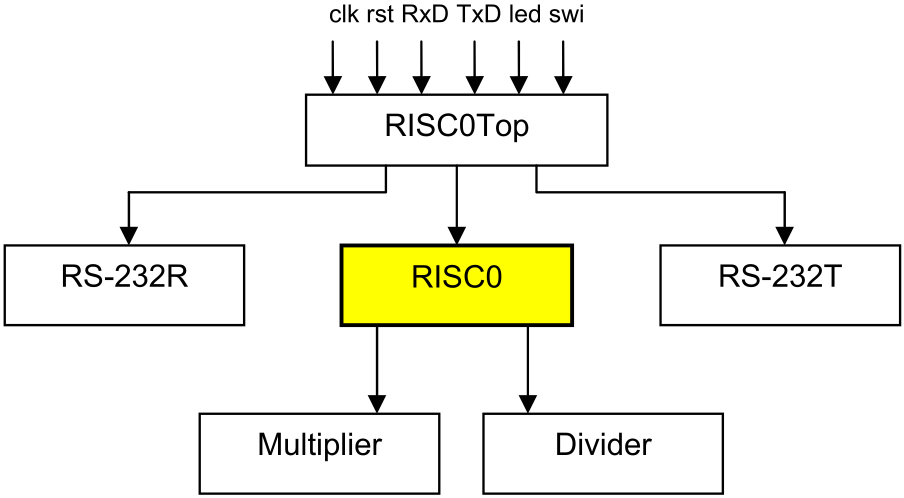
\includegraphics[width=.9\textwidth]{i/5.png}
  \caption{Block diagram of the RISC-0 configuration}
  \label{fig:risc0}
\end{figure}

The header of module RISC0 lists its parameters, signals to and from the “environment”:
\begin{verbatim}
  input clk, rst,
  input [31:0] inbus, codebus,
  output [11:0] adr,
  output rd, wr,
  output [31:0] outbus
\end{verbatim}

\subsection{ALU: Arithmetic Logic Unit}
As mentioned earlier, the processor is divided into two parts:
\begin{itemize}
  \item the ALU, and
  \item the Control Unit (CU).
\end{itemize}
In the block diagram of Figure \ref{fig:cpu} the ALU is to the left, the CU to the right, and
it is evident that they are connected by a few wires only.
\begin{figure}[h!]
  \centering
  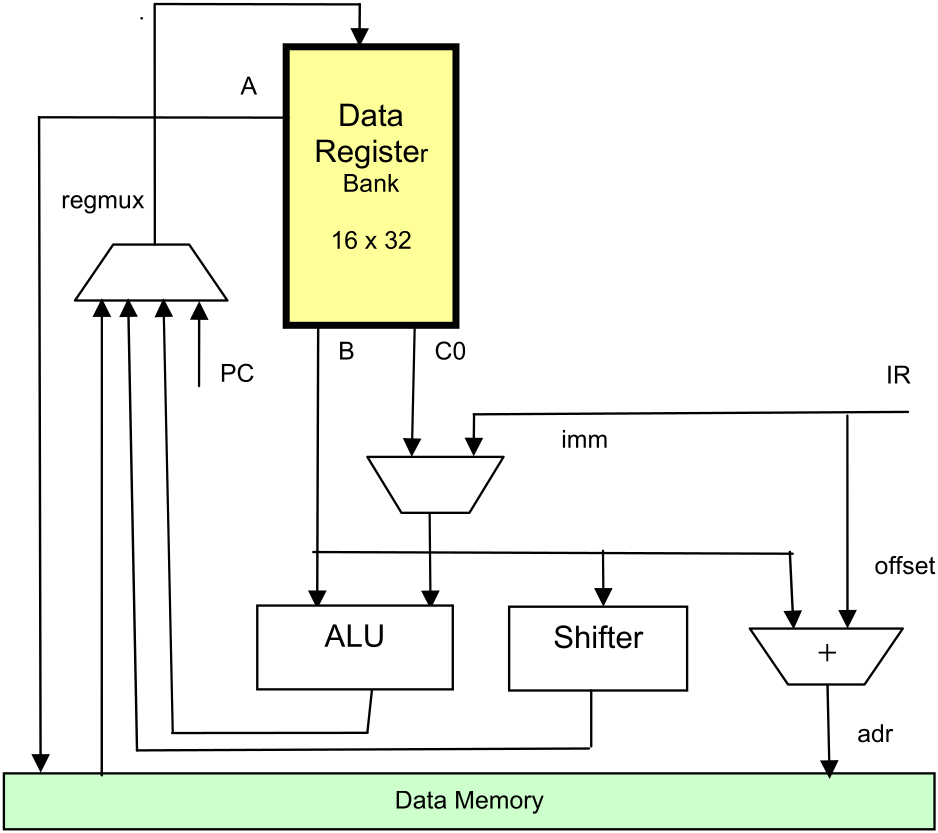
\includegraphics[width=.9\textwidth]{i/6.png}
  \caption{Block diagram of computation unit}
  \label{fig:cpu}
\end{figure}

The heart of the CPU is the bank of registers, each of the 16 registers with 32 bits. They are
represented as an array of 16 words, connected by the following signals (wires).
\begin{verbatim}
  reg[31:0] R[0:15]
 
  wire[31:0] A   // data input  (to registers)
  wire[31:0] B   // data output (from registers)
  wire[31:0] C0  // data output
 
  wire[3:0] ira0 // address of port A
  wire[3:0] irb  // address of port B
  wire[3:0] irc  // address of port C0
  wire clk       // clock
  wire regwr     // write enable
\end{verbatim}

Before proceeding, we postulate the following auxiliary signals derived from the Instruction
Register (IR), representing instruction fields and their decoding (see instruction formats
in Chapter \ref{ch:is}).
\begin{verbatim}
  IR = pmout; // instruction from Program Memory (PM)

  p = IR[31]; // instruction fields
  q = IR[30];
  u = IR[29];
  v = IR[28];
  w = IR[16];

  cc = IR[26:24];
  op = IR[19:16];

  ira = IR[27:24]:
  irb = IR[23:20];
  irc = IR[ 3: 0];
  im  = IR[15: 0];
  off = IR[19: 0]:
 
  MOV = ~p & (op ==  0); // decode signals
  LSL = ~p & (op ==  1);
  ASR = ~p & (op ==  2);
  ROR = ~p & (op ==  3);
  AND = ~p & (op ==  4);
  ANN = ~p & (op ==  5);
  IOR = ~p & (op ==  6);
  XOR = ~p & (op ==  7);
  ADD = ~p & (op ==  8);
  SUB = ~p & (op ==  9);
  MUL = ~p & (op == 10);
  DIV = ~p & (op == 11);
  LDW =  p & ~q & ~u;
  STW =  p & ~q &  u;
  BR  =  p &  q;
\end{verbatim}

From the block diagram of Figure \ref{fig:cpu} we now derive the following expressions for further signals:
\begin{verbatim}
  ira0 = (BR) ? 15 : ira; // return address of BL to R15
  C1 = ~q ? C0 : {{16{v}}, im};

  aluRes = MOV
    ? C1
    :  LSL  ? t3       // L-shifter output
    : (ASR
      |ROR) ? s3       // R-shifter output
    :  AND  ? B &  C1
    :  ANN  ? B & ~C1
    :  IOR  ? B |  C1
    :  XOR  ? B ^  C1
    :  ADD  ? B +  C1 + (u & C)
    :  SUB  ? B -  C1 - (u & C)
    :  MUL  ? product [31:0] // multiplier output
    :  DIV  ? quotient : 0;  // divider output

  regmux =                   //  register input D
    (LDW & ~ioenb) ? dmout : // from memory
    (LDW &  ioenb) ? inbus : // from input bus
    (BR & v) ? {18'b0, nxpc, 2'b0} : aluRes;
              // return address from control unit;
\end{verbatim}

In most instructions, the result $regmux$ is stored in a register. The exceptions are:
\begin{itemize}
  \item Branch instructions, unless the return address is to be saved (BR \& \textasciitilde{}u)
  \item Branch instructions whose condition is not met (BR \& \textasciitilde{}cond)
  \item Store instructions
  \item Stalls (discussed later)
\end{itemize}

Writing to registers is controlled by the signal $regwr$, defined as:
\begin{verbatim}
  regwr = (~p & ~stall) | (LDW & ~stall & ~stall1)
                        | (BR & cond & v);
\end{verbatim}

Assignment to the register bank is specified as
\begin{verbatim}
  R[ira0] <= regwr ? regmux : A;
\end{verbatim}

In addition to the data registers, 4 single-bit registers are provided to hold some predicates of
the computed result. They are traditionally called Condition Codes (CC), and they are used (tested)
by BIs. These registers are N, Z, C, V.
\begin{verbatim}
  N <= regwr ? regmux[31]  : N; // sign
  Z <= regwr ? (regmux==0) : Z; // zero
\end{verbatim}

N and Z are set by all register operations, C and V by additions and subtractions only. The values
for C and V are shown in the detailed program listings. Incidentally, C depends on its interpretation
as a carry or a borrow bit.

Parallel to the path from register output to register input through the ALU lies the path through
2 shifters, one for left and one for right. Shifters are, like circuits for logical and arithmetic
operations, entirely combinational circuits. They consist of multiplexers only. The \emph{left shift}
(LSL) feeds zero bits to the right.

A basic element on our FPGA are “lookup tables” with 4 inputs and a single output resulting from
any function of the inputs. Hence, a 4-input multiplexer is the preferred element. In order to be
able to shift by any amount between 0 and 31, 3 stages are required. The 1st shifts by 0, 1, 2, or
3 bits, the 2nd by 0, 4, 8, or 12 bits, and the 3rd by 0 or 16 bits. The following signals are
involved (the shift count is split):
\begin{verbatim}
  wire[31:0] t1,t2,t3, s1,s2,s3; wire[1:0] sc1, sc0;
                                     // shift counts
  assign sc0 = C1[1:0]:
  assign sc1 = C1[3:2];
\end{verbatim}

The shifter input is B, output for LSL is t3. The intermediates between multiplexers are t1 and t2: 
\begin{verbatim}
  assign t1 = (sc0==3) ? { B[28:0],  3'b0} :
              (sc0==2) ? { B[29:0],  2'b0} :
              (sc0==1) ? { B[30:0],  1'b0} : B;
  assign t2 = (sc1==3) ? {t1[19:0], 12'b0} :
              (sc1==2) ? {t1[23:0],  8'b0} :
              (sc1==1) ? {t1[27:0],  4'b0} : t1;
  assign t3 =   C1[4]  ? {t2[15:0], 16'b0} : t2;
\end{verbatim}

The right shifter is quite similar (output is named s3 instead of t3). It implements both right
shift (ASR) and right rotation (ROR) (determined by $u$). Bits shifted into the left end, for
ASR, are replicas of the leftmost (sign) bit B[31], whereas for ROR, are repeatedly taken from
the rightmost:
\begin{verbatim}
 assign s1 =
  (sc0==3) ? {(u ? B[2:0] : {3{B[31]}}), B[31:3]} :
  (sc0==2) ? {(u ? B[1:0] : {2{B[31]}}), B[31:2]} :
  (sc0==1) ? {(u ? B[0] : B[31]), B[31:1]} : B;
 assign s2 =
  (sc1==3) ? {(u?s1[11:0]:{12{s1[31]}}),s1[31:12]}:
  (sci==2) ? {(u?s1[7:0]:{8{s1[31]}}),s1[31:8]}:
  (sci==1) ? {(u?s1[3:0]:{4{s1[31]}}),s1[31:4]}:s1;
 assign s3 =
  C1[4] ? {(u?s2[15:0]:{16{s2[31]}}),s2[31:16]} : s2;
\end{verbatim}
And this concludes the ALU explanation.

\subsection{DM: Data Memory}
The DM is represented in our case (RISC0) by a so-called Block RAM (BRAM), a facility provided by
the FPGA. Fortunately (newer versions of) Verilog compilers allow a memory to be specified as a
simple array, mapping the array onto a BRAM:
\begin{verbatim}
  reg[31:0] mem[size-1 : 0];

  mem[adr] <= dmin;  // outbus A
  dmout <= mem[adr];
\end{verbatim}

The memory uses the following signals:
\begin{verbatim}
  wire[31:0] dmin, dmout; // input and output ports
  wire wr;                // write enable
  wire[13:0] adr;         // memory address
 
  dmin = A;
  dmwr = STW & ~stall;
  dmadr = B[13:0] + off[13:0];
\end{verbatim}

The memory is configurable as a 2K (or 4k) block. Its elements are 32-bit words. As the RISC uses
byte addresses, the address fed to the RAM is actually dmadr[12:2], and only words, not bytes can
be accessed. Address bits 0 and 1 are ignored. (The $stall$ signal will be explained later).

\subsection{CU: Control Unit}
The CU determines the sequence of executed instructions. It contains two registers, the Program
Counter (PC) holding the address of the current instruction, and the current Instruction Register
(IR) holding the instruction currently being interpreted. Instructions are obtained from the
Program Memory (PM), also a BRAM with 2K words and the signals.
\begin{verbatim}
  wire [31:0] pmout; // output port
  wire [11:0] pcmux; // memory address
\end{verbatim}

The principal task of this unit is to generate the address of the next instruction. There are
essentially only 4 cases:
\begin{enumerate}
  \item Zero on reset;
  \item The next address is the current plus 1 (i.e. $PC+1$);
  \item Given by the instruction explicitly (BIs);
  \item Taken from a register, (which is used for returning from procedures).
\end{enumerate}

In a Harvard architecture, ALU and CU operate simultaneously. In each clock cycle, the CU fetches
the next instruction from the PM into the IR, and the ALU operates on registers or the DM. As an
example, the short instruction sequence
\begin{verbatim}
  0   ADD R0 R0 2
  1   SUB R0 R0 1
  2   B 0
\end{verbatim}
is traced as follows over 5 clock cycles:
\begin{table}[h!]
  \centering
  \begin{tabular}{l l l l}
    pcmux & IR & PC & R0 \\\hline
    0 \\
    1 & ADD & 0 & 0 \\
    2 & SUB & 1 & 2 \\
    0 & B   & 2 & 1 \\
    1 & ADD & 0 & 1 \\
    2 & SUB & 1 & 3
  \end{tabular}
\end{table}

\begin{figure}[h!]
  \centering
  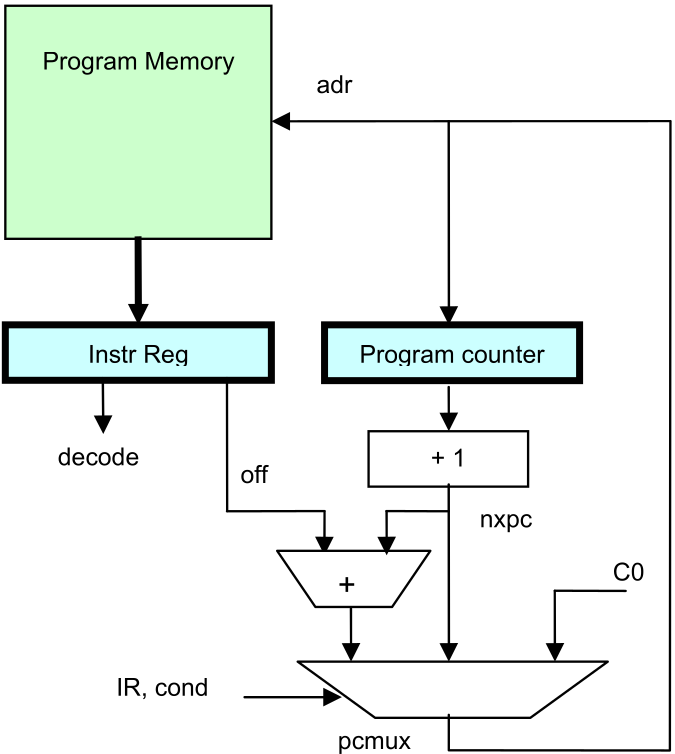
\includegraphics[width=.9\textwidth]{i/7.png}
  \caption{The control unit}
  \label{fig:cu}
\end{figure}
The CU is quite straight-forward, as show in Figure \ref{fig:cu}, and defined by the following
expressions:
\begin{verbatim}
  IR = pmout;
  nxpc = PC + 1;
  pcmux =     (~rst) ? 0  :
             (stall) ? PC : // do not advance
    (BR & cond &  u) ? off[11:0] + nxpc :
    (BR & cond & ~u) ? C0[13:2]         : nxpc;
 
  always @(posedge clk) PC <= pcmux; end
\end{verbatim}

Here we notice that all BIs are subject to a condition. The condition is specified by the condition
field of the instruction and is a logical function of the 4 condition registers N, Z, C, V. The
signal $cond$ is defined as
\begin{verbatim}
  cond = IR[27] ^        // IR[27] inverts sense
    ((cc == 0) &     N | // MI, PL
     (cc == 1) &     Z | // EQ, NE
     (cc == 2) &     C | // CS, CC
     (cc == 3) &     V | // VS, VC
     (cc == 4) & (C|Z) | // LS, HI
     (cc == 5) &     S | // LT, GE
     (cc == 6) & (S|Z) | // LE, GT
     (cc == 7));         //  T, F
\end{verbatim}

The memory block of the FPGA already contains an output register. For this reason IR is actually
declared as a wire, but not as a register (which is represented by $pmout$). Note that the memory
has $clk$ as an input signal. This seemingly trivial and incidental detail has yet another
consequence. As the address signal travels through the decoder and the selected value proceeds to
this output register, the read value is actually available only in the next cycle after the address
was applied to the memory. This implies that actually the reading of a value takes 2 cycles. This
contradicts the rule that in RISCs every instruction be executed in a single cycle. However, memory
access is considered as a special case, and provisions must be made to allow it to take longer.

The device to solve this problem is \emph{stalling} the processor, i.e. to retain it in the same
state over 2 or more cycles. This is achieved by simply generating a $stall$ signal which, if
active, feeds PC itself to the multiplexer. In our case, this signal must arise when a LD
instruction is present, and it must remain active for exactly one clock period. This is achieved
by the following circuit with signals shown in Figure \ref{fig:stall}:
\begin{verbatim}
  reg stall1;
  wire stall, stallL;
 
  stall = stallL;
  stallL = LDW & ~stall1;
  stall1 <= stallL;
\end{verbatim}
\begin{figure}[h!]
  \centering
  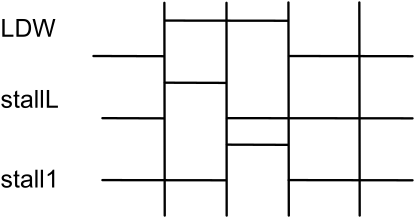
\includegraphics[width=.9\textwidth]{i/8.png}
  \caption{Stall generation for memory access}
  \label{fig:stall}
\end{figure}
This circuit actually represents a very simple state machine.
 
\subsection{multiplier}
Multiplication is an inherently more complex operation than either addition or subtraction. After
alll, multiplication can be composed (of a sequence) of additions. There are many methods to
implement multiplication, all based on the same concept of a series of additions. They show the
fundamental problem of trade-off between time and space (circuitry). Some solutions operate with
a minimum of additional circuitry — actually without — but sacrifice speed. These are the
implementations in software. Naturally, they perform the necessary additions in sequence. The
partial sums are stored in variables. At the other end of the spectrum lie solutions which use a
multitude of adders operating concurrently. They are fast, but the amount of required circuitry is
high.

Here we present a middle solution. It needs a single adder only and performs additions in sequence,
with partial sums stored in a special register. The sequence of additions is triggered by a single
multiply instruction, which makes this solution still faster than a pure software solution, which
would typically be presented as a procedure.

Let us briefly recapitulate the basics of a multiplication $p := x y$. Here $p$ is called the
product, $x$ the multiplier, and $y$ the multiplicand. Let $x$ and $y$ be unsigned integers.
Consider $x$ in binary form:
\[ x = x_{31}2^{31} + x_{30}2^{30} +...+ x_12^1 + x_02^0 \]

We obtain the product by a sequence of 32 additions, each term of the form $x_k2^ky$, i.e. of $y$
left shifted by $k$ positions multiplied by $x_k$. Since $x_k$ is either 0 or 1, the term is either
0 or $y$. Multiplication is thus performed by an adder and a selector. Instead of using $x$, as a
selector value, $A$ (initially equal to $x$) is shifted right in each so-called \emph{add-shift}
step, so that $A_0$ is always the selector. It is represented by $ODD(A)$. The algorithm is shown
by the following piece of program. $B$ must be a variable of double length:
\begin{verbatim}
  B := 0; A := x; i := 0;

  REPEAT
    IF ODD(A) THEN B := B+y; A := A-1 END;
    B := 2 * B; A := A DIV 2; i := i+1
  UNTIL i = 32
\end{verbatim}

The invariant $Ay + B = xy$ is maintained over the iterations, and at the end $A = 0$, yielding the
desired result $B = xy$. $A := A\!-\!1$ can be omitted due to the subsequent division.

Let us now transpose this algorithm into hardware. Instead of shifting $B$ to the left, we shift it
to the right, adding $y$ to B's upper half. This has the advantage of using the concatenated $B$ and
$A$, denoted as $P$ (product), as a double register. In step $i$, $P[63:32-i]$ is the partial
product, and $P[31-i:0]$ is the multiplier. The size of the multiplier decreases by 1 in each step,
whereas the size of the product increases by 1.

The multiplier is controlled by a rudimentary state machine S, actually a simple counter running
from 0 to 32. Step 0 is for initialization. The multiplier is shown schematically in Figure \ref{fig:multiplier}.
\begin{figure}[h!]
  \centering
  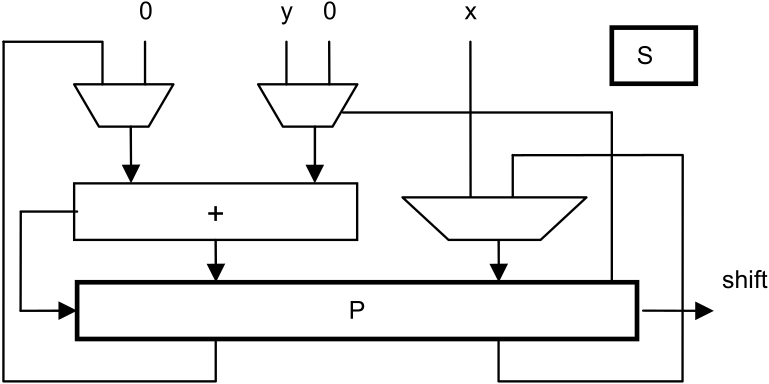
\includegraphics[width=.9\textwidth]{i/9.png}
  \caption{Schematic of multiplier}
  \label{fig:multiplier}
\end{figure}

The multiplier interprets its operands as signed ($u = 0$) or unsigned ($u = 1$) integers. The
difference between unsigned and signed representation is that in the former case the most
significant term has a negative weight ($-x_{31}2^{31}$). Therefore, implementation of signed
multiplication requires very little change: Term 31 is subtracted instead of added (see
complete program listing below).
\begin{figure}[h!]
  \centering
  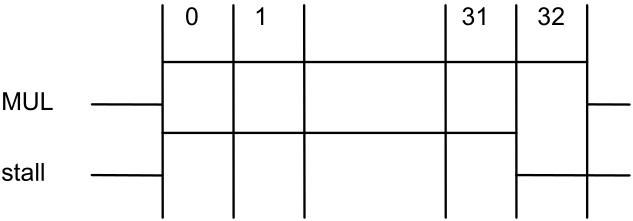
\includegraphics[width=.9\textwidth]{i/a.png}
  \caption{Generating stall}
  \label{fig:gs}
\end{figure}

During execution of the 32 add-shift steps the processor must be stalled. The process proceeds
and the counter $S$ advances as long as the input MUL is active (high). MUL indicates that the
current operation is a multiplication, and the signal is stable until the processor advances to
the next instruction. This happens when step 31 is reached:
\begin{verbatim}
  stall = MUL & ~(S == 33);
  S <= MUL ? S+1: 0;
\end{verbatim}

The complete multiplier is listed below, $u = 0$ specifies singned, $u = 1$ unsigned operands:
\begin{verbatim}
  module Multiplier(
    input clk, run, u,
    output stall,
    input [31:0] x, y,
    output[63:0] z
  );
  reg[ 5:0] S;    // state
  reg[63:0] P;    // product
  wire[31:0] w0;
  wire[32:0] w1;
  
  assign stall = run & ~(S == 33);
  assign w0 = P[0] ? y : 0;
  assign w1 = (S==32)&u ? {P[63],P[63:32]}-{w0[31],w0}
                        : {P[63],P[63:32]}+{w0[31],w0};
  assign z = P;
 
  always @ (posedge(clk)) begin
    P <= (S == 0) ? {32'b0, x}: {w1[32:0], P[31:1]};
    S <= run ? S+1 : 0;
  end
  endmodule
\end{verbatim}

Implementing multiplication in hardware made the operation about 30 times faster than its solution
by software. A significant factor! As multiplication is a relatively rare operation — at least in
comparison with addition and subtraction — early RISC designs (MIPS, SPARC, ARM) refrained from its
full implementation in hardware. Instead, an instruction called \emph{multiply} step was provided,
performing a single add-shift step. A multiplication was then programmed by a sequence of 32 step
instructions, typically provided as a subroutine.

\subsection{divider}
Division is similar to multiplication in structure, but even slightly more complicated. We present
its implementation by a sequence of 32 \emph{shift-subtract} steps, the complement of add-shift.
Here we discuss division of unsigned integers only with the following definitions. $x$ is the
dividend, $y$ the divisor.
\[ q = x\text{ DIV }y\text{  }r = x\text{ MOD }y \]

where $q$ is the quotient, $r$ the remainder, satisfying
\[ x = qy + r\text{ with }0 \le r < y \]

The division algorithm is shown by the following piece of program with variables $R$ and $Q$:
\begin{verbatim}
  R := x; Q := 0; i := 0;
  REPEAT R := R DIV 2; Q := 2*Q; i := i+1;
    IF R>=y THEN R := R-y; Q := Q+1 END
  UNTIL i = 32
\end{verbatim}

The invariants $Qy + R = x$ and $0 \le R < y2^{32-i}$ are maintained over the iterations, with
$i = 32$ yielding the desired result.

When transposing the algorithm into hardware, we use the same trick of using a double register
RQ as in multiplication. Initially we set RQ to $x$, the dividend, and then subtract multiples of $y$ from
it, each time checking that the result is not negative. Initially, $R$ may be a 64-bit value
initially; its size decreases by 1 in each step. $Q$ is initially 0, and its size increases by 1 in
each step. $(R, Q[31:i])$ holds the remainder, $Q[i-1:0]$ holds the quotient.
\begin{figure}[h!]
  \centering
  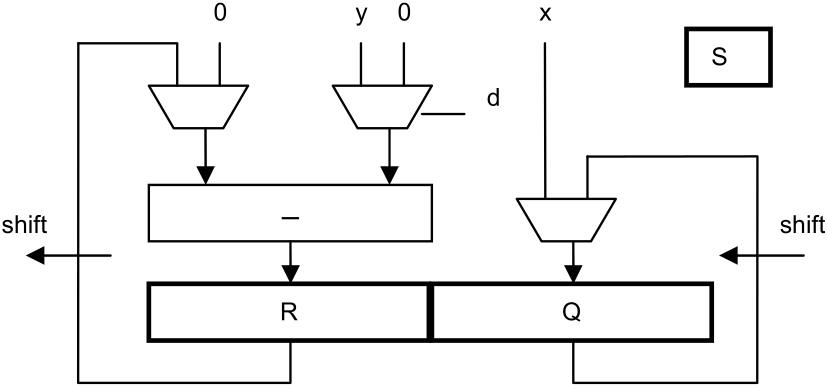
\includegraphics[width=.9\textwidth]{i/b.png}
  \caption{Schematic of divider}
  \label{fig:divider}
\end{figure}

Stall generation is the same as for the multiplier. Further details are shown in the subsequent
program listing.
\begin{verbatim}
  module Divider(
    input clk, run, u,
    output stall,
    input [31:0] x, y,        // y > 0
    output[31:0] quot, rem
  );
  reg [ 5:0] S;               // state
  reg [63:0] RQ;
  wire       sign;
  wire[31:0] x0, w0, w1;
 
  assign stall = run & ~(S == 33);
  assign sign = x.31 & u;
  assign x0 = sign ? -x : x;
  assign w0 = RQ[62:31];
  assign w1 = w0 - y;
 
  always @(posedge(clk)) begin
    RQ <= (S == 0) ? {32'b0, x0} :
          {(w1[31] ? w0 : w1), RQ[30:0], ~w1[31]}:
    S <= run ? S+1 : 0;
  end
 
  assign quot = sign ? -RQ[31:0] - 1 : RQ[31:0];
  assign rem  = sign ? y - RQ[63:32] : RQ[63:32];
  endmodule
\end{verbatim}

\subsection{environment}
Module RISC0 is imported by RISC0Top, which thereby represents the processors environment. Apart
from providing clock and reset signals, it connects various devices with the processor’s input and
output busses, and selects them according to the I/O address. These devices are:
\begin{enumerate}
  \item A counter incremented every millisecond ($adr: 0$)
  \item A set of 8 dip switches ($adr: 4$)
  \item A set of 8 Light Emitting Diodes (LED) ($adr: 4$)
  \item An RS-232 receiver (serial data line) ($adr: 8, 12$)
  \item An RS-232 transmitter ($adr: 8, 12$)
\end{enumerate}

The RS-232 receiver and transmitter are described in subsequent sections, the top module itself is
listed here with the omission of clock generation. The clock frequency is 35 MHz. The signals in its
heading refer to off-chip components (see also Figure \ref{fig:risc0}).
\begin{verbatim}
  module RISC0Top(
    input       CLK50M, rstin, RxD,
    input [7:0] swi,
    output[7:0] leds,
    output      TxD
  );
  wire clk, clkLocked;
  reg rst;
 
  wire[ 5:0] ioadr;
  wire[ 3:0] iowadr;
  wire       iowr;
  wire[31:0] inbus, outbus;
 
  wire[ 7:0] dataTx, dataRx;
  wire       rdyRx, doneRx, startTx, rdyTx;
  wire       limit;              // of cnt0
 
  reg[ 7:0] Lreg;
  reg[15:0] cnt0;
  reg[31:0] cnt1;                // milliseconds
 
  RISC0 riscx(.clk(clk), .rst(rst), .iord(iord),
              .iowr(iowr), .ioadr(ioadr),
              .inbus(inbus), .outbus(outbus)):
  RS232R receiver(.cik(clk), .rst(rst), .RxD(RxD),
                  .done(doneRx), .data(dataRx),
                  .rdy(rdyRx));
  RS232T transmitter(.clk(clk), .rst(rst),
                     .start(startTx), .data(dataTx),
                     .TxD(TxD), .rdy(rdyTx));

  assign iowadr = ioadr[5:2];
  assign inbus = (iowadr==0) ? cnt1 :
                 (iowadr==1) ? swi  :
                 (iowadr==2) ? {24'b0, dataRx} :
                 (iowadr==3) ? {30'b0, rdyTx, rdyRx}
                             : 0;

  assign dataTx  = outbus[7:0];
  assign startTx = iowr & (iowadr == 2);
  assign doneRx  = iord & (iowadr == 2):
  assign limit   = (cnt0 == 35000);
  assign leds    = Lreg;
 
  always @(posedge clk) begin
    rst  <= ~rstin & clkLocked;
    Lreg <= ~rst ? 0 : (iowr & (iowadr == 1))
                     ? outbus[7:0] : Lreg;
    cnt0 <= limit ? 0 : cnt0 + 1;
    cnt1 <= limit ? cnt1 + 1 : cnt1;
  end
  endmodule
\end{verbatim}

\subsection{transmitter}
RS-232 is an old standard for serial data transmission. We chose to describe it here because of its
inherent simplicity. The data are transmitted in packets of a fixed length, here of length 8, i.e.
byte-wise. Bytes are transmitted asynchronously. Their beginning is marked by a start-bit, and at
the end a stop-bit is appended. Hence, a packet is 10 bits long (see Figure \ref{fig:rs232}).
Within a packet, transmission is synchronous, i.e. with a fixed clock rate, on which transmitter
and receiver agree. The standard defines several packet lengths and many clock rates. Here we use
19200 bit/s.
\begin{figure}[h!]
  \centering
  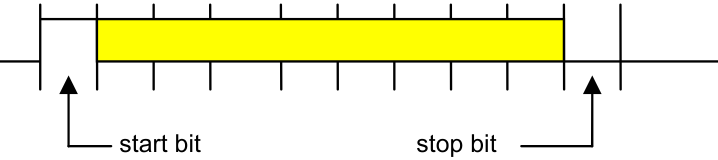
\includegraphics[width=.9\textwidth]{i/c.png}
  \caption{RS-232 packet format}
  \label{fig:rs232}
\end{figure}

The input signal start triggers the state machine by setting register $run$. The transmitter has 2
counters and a shift register. Counter $tick$ runs from 0 to 1823, yielding a frequency of .35’000
/ 1823 = 19.2 KHz, the transmission rate for bits. The signal $endtick$ advances counter $bitcnt$,
running from 0 to 9 (the number of bits in a packet). Signal $endbit$ resets $run$ and the counter
to 0. Signal $rdy$ indicates whether or not a next byte can be loaded and sent.
\begin{verbatim}
  module RS232T(
    input      clk, rst,
    input      start, // request to accept & send a byte
    input[7:0] data,
    output     rdy,   // status
    output     TxD    // serial data
  );
  wire endtick, endbit;
  reg       run;
  reg[11:0] tick;
  reg[ 3:0] bitcnt;
  reg[ 8:0] shreg;

  assign endtick = tick==1823;
  assign endbit  = bitcnt==9;
  assign rdy = ~run;
  assign TxD = shreg[0];

  always @(posedge clk) begin
    run <= (~rst | endtick & endbit) ? 0 :
                               start ? 1 : run;
    tick <= (run & ~endtick) ? tick + 1 : 0;
    bitcnt <= (endtick & ~endbit) ? bitcnt + 1 :
              (endtick &  endbit) ? 0 : bitcnt;
    shreg <= (~rst) ? 1 : start ? {data, 1'b0} :
            endtick ? {1'b1, shreg[8:1]} : shreg;
  end
  endmodule
\end{verbatim}

\subsection{receiver}
The RS-232 receiver is structured very similarly with 2 counters and a shift register. The state
machine is triggered by an incoming start bit at $RxD$. For the purpose of robustness, a
synchronizer and edge detector are provided for the incoming signal. The state $rdy$ is set when
the last data bit has been received, and it is reset by the $done$ signal, generated when reading
a byte. The input is sampled in the middle of the bit period rather than at the end, namely when
$midtick = endtick/2$.
\begin{verbatim}
  module RS232R(
    input clk, rst, RxD,
    input       done, // "byte has been read"
    output      rdy,
    output[7:0] data
  );
  wire endtick, midtick;
  reg       run, stat;
  reg       Q0, Q1; // synchronizer & edge detector
  reg[11:0] tick;
  reg[ 3:0] bitcnt;
  reg[ 7:0] shreg;

  assign endtick = tick==1823;
  assign midtick = tick== 911;
  assign endbit  = bitcnt== 8;
  assign data = shreg;
  assign rdy  = stat;

  always @ (posedge clk) begin
    Q0 <= RxD; Q1 <= Q0;
    run <= (Q1 & ~Q0) ? 1 :
           (~rst | endtick & endbit) ? 0 : run;
    tick <= (run & ~endtick) ? tick + 1 : 0;
    bitcnt <= (endtick & ~endbit) ? bitcnt+1 :
              (endtick &  endbit) ? 0 : bitcnt;
    shreg <= midtick ? {Q1, shreg[7:1]} : shreg;
    stat <= (endtick & endbit) ? 1 :
                 (~rst | done) ? 0 : stat;
  end
  endmodule
\end{verbatim}
